\documentclass{article}  
% Include all project wide packages here.
\usepackage{fullpage}
\usepackage{polyglossia}
\setmainlanguage{dutch}
\usepackage{csquotes}
\usepackage{graphicx}
\usepackage{epstopdf}
\usepackage{pdfpages}
\usepackage{caption}
\usepackage[list=true]{subcaption}
\usepackage{float}
%\usepackage{mathtools}
\usepackage{standalone}
\usepackage{import}
\usepackage{tocloft}
\usepackage{wrapfig}
\usepackage{authblk}
\usepackage{array}
\usepackage{booktabs}
\usepackage[toc,page,title,titletoc]{appendix}
\usepackage{xunicode}
\usepackage{amsmath}
\usepackage{fontspec}
\usepackage{unicode-math}
\usepackage[
    backend=bibtexu,
	texencoding=utf8,
bibencoding=utf8,
    style=ieee,
    sortlocale=nl_NL,
    language=auto
]{biblatex}
\usepackage{listings}
\newcommand{\includecode}[3][c]{\lstinputlisting[caption=#2, escapechar=, style=#1]{#3}}
\newcommand{\superscript}[1]{\ensuremath{^{\textrm{#1}}}}
\newcommand{\subscript}[1]{\ensuremath{_{\textrm{#1}}}}


\newcommand{\chapternumber}{\thechapter}
\renewcommand{\appendixname}{Bijlage}
\renewcommand{\appendixtocname}{Bijlagen}
\renewcommand{\appendixpagename}{Bijlagen}

\usepackage[hidelinks]{hyperref} %<--------ALTIJD ALS LAATSTE
  
\renewcommand{\familydefault}{\sfdefault}

\setmainfont[Ligatures=TeX]{Myriad Pro}
\setmathfont{Asana Math}
\setmonofont{Lucida Console}

\usepackage{titlesec, blindtext, color}
\definecolor{gray75}{gray}{0.75}
\newcommand{\hsp}{\hspace{20pt}}
\titleformat{\chapter}[hang]{\Huge\bfseries}{\chapternumber\hsp\textcolor{gray75}{|}\hsp}{0pt}{\Huge\bfseries}
\renewcommand{\familydefault}{\sfdefault}
\renewcommand{\arraystretch}{1.2}
\setlength\parindent{0pt}

%For code listings
\definecolor{black}{rgb}{0,0,0}
\definecolor{browntags}{rgb}{0.65,0.1,0.1}
\definecolor{bluestrings}{rgb}{0,0,1}
\definecolor{graycomments}{rgb}{0.4,0.4,0.4}
\definecolor{redkeywords}{rgb}{1,0,0}
\definecolor{bluekeywords}{rgb}{0.13,0.13,0.8}
\definecolor{greencomments}{rgb}{0,0.5,0}
\definecolor{redstrings}{rgb}{0.9,0,0}
\definecolor{purpleidentifiers}{rgb}{0.01,0,0.01}


\lstdefinestyle{csharp}{
language=[Sharp]C,
showspaces=false,
showtabs=false,
breaklines=true,
showstringspaces=false,
breakatwhitespace=true,
escapeinside={(*@}{@*)},
columns=fullflexible,
commentstyle=\color{greencomments},
keywordstyle=\color{bluekeywords}\bfseries,
stringstyle=\color{redstrings},
identifierstyle=\color{purpleidentifiers},
basicstyle=\ttfamily\small}

\lstdefinestyle{c}{
language=C,
showspaces=false,
showtabs=false,
breaklines=true,
showstringspaces=false,
breakatwhitespace=true,
escapeinside={(*@}{@*)},
columns=fullflexible,
commentstyle=\color{greencomments},
keywordstyle=\color{bluekeywords}\bfseries,
stringstyle=\color{bluestrings},
identifierstyle=\color{purpleidentifiers}
}

\lstdefinestyle{vhdl}{
language=VHDL,
showspaces=false,
showtabs=false,
breaklines=true,
showstringspaces=false,
breakatwhitespace=true,
escapeinside={(*@}{@*)},
columns=fullflexible,
commentstyle=\color{greencomments},
keywordstyle=\color{bluekeywords}\bfseries,
stringstyle=\color{redstrings},
identifierstyle=\color{purpleidentifiers}
}

\lstdefinestyle{xaml}{
language=XML,
showspaces=false,
showtabs=false,
breaklines=true,
showstringspaces=false,
breakatwhitespace=true,
escapeinside={(*@}{@*)},
columns=fullflexible,
commentstyle=\color{greencomments},
keywordstyle=\color{redkeywords},
stringstyle=\color{bluestrings},
tagstyle=\color{browntags},
morestring=[b]",
  morecomment=[s]{<?}{?>},
  morekeywords={xmlns,version,typex:AsyncRecords,x:Arguments,x:Boolean,x:Byte,x:Char,x:Class,x:ClassAttributes,x:ClassModifier,x:Code,x:ConnectionId,x:Decimal,x:Double,x:FactoryMethod,x:FieldModifier,x:Int16,x:Int32,x:Int64,x:Key,x:Members,x:Name,x:Object,x:Property,x:Shared,x:Single,x:String,x:Subclass,x:SynchronousMode,x:TimeSpan,x:TypeArguments,x:Uid,x:Uri,x:XData,Grid.Column,Grid.ColumnSpan,Click,ClipToBounds,Content,DropDownOpened,FontSize,Foreground,Header,Height,HorizontalAlignment,HorizontalContentAlignment,IsCancel,IsDefault,IsEnabled,IsSelected,Margin,MinHeight,MinWidth,Padding,SnapsToDevicePixels,Target,TextWrapping,Title,VerticalAlignment,VerticalContentAlignment,Width,WindowStartupLocation,Binding,Mode,OneWay,xmlns:x}
}

%defaults
\lstset{
basicstyle=\ttfamily\small,
extendedchars=false,
numbers=left,
numberstyle=\ttfamily\tiny,
stepnumber=1,
tabsize=4,
numbersep=5pt
}  
\begin{document}

\newcommand{\tss}{\textsubscript}
\newcommand{\tsss}{\textsuperscript}

Voor het bepalen van de \emph{R\tss{eq}} en de \emph{C\tss{out}} wordt er gebruikt gemaakt van een SPICE model en enkele berekeningen. Een vereenvoudigde schakeling om de \emph{C\tss{out}} te bepalen is te zien in figuur \ref{res:PDN_schematic}. Het bepalen van deze weerstand en deze capaciteit wordt gedaan aan de hand van het volgende stappenplan:

 \begin{figure} [h!]
 \begin{center}
 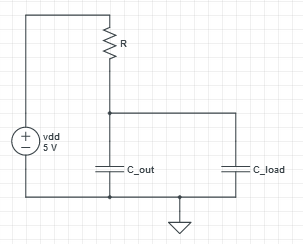
\includegraphics [scale = 0.5] {figures/PDN_schematic}
 \caption{Vereenvoudigde schakeling van het PDN, op \emph{t = 0} is de spanning over \emph{C\tss{load}} gelijk aan \emph{5V}}
 \label{res:PDN_schematic}
 \end{center}
 \end{figure}

\begin{enumerate}

%%%STAP 1%%%
\item \textbf{Stroom bepalen door NMOS transistoren op \emph{t = 0} d.m.v. SPICE simulatie}\\
Om \emph{R\tss{eq}} te bepalen moet de stroom door de NMOS transistoren worden bepaald op \emph{t = 0}. Op dit tijdstip zal, wanneer \emph{V\tss{in} = V\tss{DD}} en de spanning over \emph{C\tss{load}} gelijk is aan \emph{5V}, het PUN dicht zijn en het PDN open zijn.  De capaciteiten \emph{C\tss{load}} en \emph{C\tss{out}} zijn op dat tijdstip opgeladen en zullen zich langzaam ontladen. De \emph{R\tss{eq}} kan dan worden bepaald aan de hand van de volgende formule:

\begin{equation}
R\tss{eq} = \frac{5V}{i(0)}
\end{equation}

Hierbij is aangenomen dat R\tss{eq} op dat tijdstip constant is.

%%%STAP 2%%%
\item \textbf{De RC tijd bepalen}\\
Om de RC tijd ($\tau$) uit figuur \ref{res:PDN_schematic} te bepalen, moeten we eerst voor beide schakelingen een functie voor de spanning bepalen. Dit kan aan de hand van de volgende formule uit het Lineaire Schakelingen boek [2], p. 307:

\begin{equation}
v(t) = v(\infty) + [v(0+) - v(\infty)]e\tsss{-t/$\tau$}
\end{equation}

Als we deze formule invullen krijgen we:

\begin{equation}
v(t) = 5V \cdot e\tsss{-t/$\tau$}
\end{equation}

Als we deze formules omschrijven krijgen we:

\begin{equation}
\tau = R\tss{eq}C\tss{eq} = \frac{-t}{ln(\frac{v(t)}{5V})}
\end{equation}

Hierbij kan de waarde \emph{t} en de waarde \emph{v(t)} uit de spannings karakteristiek worden afgelezen, die is opgesteld tijdens de SPICE simulatie.

%%%STAP 3%%%
\item \textbf{\emph{C\tss{out}} berekenen aan de hand van $\tau$}\\
Als laatst kan de \emph{C\tss{out}} en berekend worden d.m.v. de RC tijd:

\begin{equation}
\tau = R\tss{eq}C\tss{eq} = R\tss{eq}(C\tss{out} + C\tss{load})
\end{equation}

Als we deze formule omschrijven krijgen we een functie die de \emph{C\tss{out}} kan bepalen:

\begin{equation}
C\tss{out} = \frac{-t}{R\tss{eq} ln(\frac{v(t)}{5V})} - C\tss{load}
\end{equation}

\end{enumerate}

\end{document}